\chapter{自發超對稱破缺與第一個\texorpdfstring{\(SU(5)\)}{SU(5)}多重態}

\lectureoverview{對稱性破缺首先呈現為譜上的可觀察現象：旋轉不變的原子具有簡併的角動量能階，而磁場會使這些能階分裂。鐵磁體則帶出更微妙的教訓：方程可以保有真空本身不具備的對稱性。無能隙磁振子、條件\(J|0\rangle\neq0\)以及非零序參量，是同一現象的三種描述。我們將此模式帶入手徵超對稱場論，藉由消去輔助場\(F\)導出標量勢\(V=|W'|^2\)，並區分超對稱真空與\(F\)破缺真空。由此得到的真空能、玻色子--費米子質量分裂、戈德斯通微子、隱藏部門與超希格斯機制，構成超對稱部分的完整討論。最後轉向大統一：\(SU(3)\times SU(2)\times U(1)\)以分塊形式嵌入\(SU(5)\)；其中第一個物質多重態由一個輕子二重態和三個反下夸克組成。}

\section{譜會留下對稱性的印記}

從原子談起，目的不只是複習初等量子力學。能階與粒子質量同屬譜資料。若對稱性使原子能階簡併，對稱性破缺便可能使能階分裂；在場論中，相應的說法是粒子多重態中的成員可能具有不同質量。

設原子態的總角動量為\(j\)，包括自旋與軌道角動量的貢獻。相對於任意選定的軸，
\begin{equation}
J_z|j,m\rangle=m\hbar|j,m\rangle,
\qquad
m=-j,-j+1,\ldots,j,
\end{equation}
因此共有\(2j+1\)個態。教科書中常見的箭頭，不應解讀成角動量向量在空間中真的只有\(2j+1\)種可能方向。量子化的是角動量沿所選軸的分量。

在空無一物且旋轉不變的空間中，沒有物理理由偏好某個軸。旋轉會混合自旋為\(j\)的多重態中的各個態，而哈密頓量的不變性意味著
\begin{equation}
[H,\mathbf J]=0,
\qquad
E_{j,-j}=E_{j,-j+1}=\cdots=E_{j,j}.
\label{eq:l9-degeneracy}
\end{equation}

\begin{classroomqa}
\audiencequestion{什麼對稱性保證，旋轉整個原子不會改變它的能量？\lecturetimestamp{00:05:53}}
\lecturerresponse{旋轉對稱性。旋轉會將角動量的一種取向變為另一種，卻不改變物理系統，因此所有\(2j+1\)個態的能量都相同。}
\end{classroomqa}

現在施加磁場\(\mathbf B=B\hat{\mathbf z}\)。相互作用
\begin{equation}
H_B=-\boldsymbol{\mu}\cdot\mathbf B
\end{equation}
會使平行於磁場的分量具有不同地位。概略而言，
\begin{equation}
\Delta E_m\propto mB.
\label{eq:l9-zeeman}
\end{equation}
在弱磁場下，不同\(m\)值的能階會線性分裂，它們之間的躍遷也會使譜線分裂。

\begin{classroomqa}
\audiencequestion{原子能階在磁場中的分裂稱為什麼？\lecturetimestamp{00:07:13}}
\lecturerresponse{塞曼效應。這是整個討論的典型例子：對稱性所造成的能階簡併，會在背景場破壞該對稱性時解除。}
\end{classroomqa}

\begin{center}
\begin{tikzpicture}[x=1.05cm,y=0.75cm,>=Latex]
  \draw[thick] (-3,0) -- (-1,0);
  \node[left] at (-3,0) {\(B=0\)};
  \foreach \y/\m in {-1.2/-1,-0.4/0,0.4/1,1.2/2} {
    \draw[thick,teal!70!black] (1,\y) -- (3,\y);
    \node[right] at (3,\y) {\(m=\m\)};
  }
  \draw[->,thick] (-0.5,0) -- (0.6,0);
  \node[above] at (0.05,0) {\(\mathbf B\neq0\)};
\end{tikzpicture}
\end{center}

\section{鐵磁體：定律具有對稱性，真空卻不然}

一個簡單的鐵磁體微觀模型，是在每個格點放置一個小磁矩。若相鄰磁矩平行排列會降低能量，低溫相便是鐵磁相。若反平行排列較受偏好，則形成反鐵磁相。強烈的熱漲落或量子漲落也可能抹去淨磁化。

假設鐵磁體充滿整個世界，並穩定在磁矩一致排列的狀態。它的內部磁場會像外加磁場一樣，使原子能階分裂。但兩者有一個關鍵差異：底層相互作用並不偏好北方、東方或任何其他方向。所有一致旋轉後的構型能量都相同：
\begin{equation}
\mathbf M(\mathbf x)=M_0\hat{\mathbf n},
\qquad
\hat{\mathbf n}\in S^2.
\label{eq:l9-ferromagnetic-vacua}
\end{equation}
方程具有旋轉不變性，但實際的基態選定了一個\(\hat{\mathbf n}\)。這是自發對稱性破缺，而非顯式對稱性破缺。

由這種介質中的激發構成的居民，無法抓住整個宇宙並使它旋轉。因此在局部觀察下，所選方向看起來就像外加磁場所指定的方向一樣基本。原子仍呈現相同的能階排列，角動量是沿著\(\hat{\mathbf n}\)而非外部指定的\(z\)軸來分類。問題是，內部觀察者如何得知這種表面上的不對稱來自狀態，而非定律。

\subsection{戈德斯通判據}

所有磁矩一致旋轉，便會從式~\eqref{eq:l9-ferromagnetic-vacua}所示的一個真空轉到另一個真空，而且不需耗費能量。現在讓取向在空間中緩慢變化。相鄰磁矩會彼此牽引，使這種形變以自旋波的形式傳播；自旋波的量子就是磁振子。波長趨近無窮大時，構型便趨近一致旋轉，因此激發能也趨近於零：
\begin{equation}
k=\frac{2\pi}{\lambda}\longrightarrow0
\quad\Longrightarrow\quad
E(k)\longrightarrow0.
\label{eq:l9-gapless-magnon}
\end{equation}
兩位居民可以擾動附近的磁矩，讓這種波在介質中傳播，並測量任意低的能量。即使他們無法旋轉整個世界，這項實驗仍能揭示自發對稱性破缺。

\editorialnote{鐵磁體中的磁振子雖然無能隙，色散關係通常是非相對論性的二次形式\(E\propto k^2\)，而非相對論關係\(E\propto|k|\)。講課中所說的「無質量」，是指具有物理意義的能隙為零。兩者都是戈德斯通模。}

同樣的概念也適用於連續內部對稱性，包括粒子物理中的規範群與味群。然而，當遭到破缺的對稱性是規範對稱性時，戈德斯通模不會以獨立無質量粒子的形式保留下來。

\begin{classroomqa}
\audiencequestion{自發對稱性破缺與規範不變性結合時，會發生什麼事？\lecturetimestamp{00:15:56}}
\lecturerresponse{戈德斯通玻色子會為規範場提供額外的極化態，使規範玻色子獲得質量；這就是希格斯機制，我們之後會在引力的類比中再談到它。}
\end{classroomqa}

\section{對稱性破缺的三種等價表徵}

現在可以用三種彼此呼應的方式來描述鐵磁體。

\paragraph{簡併真空。}
每個取向\(\hat{\mathbf n}\)都對應一個最低能量態。雖然對稱性將這些真空彼此聯繫，物理實際發生在這個族群中被選定的一個態。

\paragraph{不湮滅真空的生成元。}
設\(J_a\)為旋轉生成元。有限變換為
\begin{equation}
U(\epsilon)=e^{-i\epsilon J_a},
\end{equation}
其中\(J_a|0\rangle\)正比於真空的無窮小變化，而非整個旋轉後的態。

\begin{classroomqa}
\audiencequestion{旋轉對稱性的生成元是什麼？\lecturetimestamp{00:17:29}}
\lecturerresponse{總角動量的各個分量。我們稱它們為\(J_a\)，因為它們會旋轉態中的所有成分，而不只是某個原子。}
\end{classroomqa}

未破缺的生成元滿足
\begin{equation}
J_a|0\rangle=0.
\label{eq:l9-unbroken-generator}
\end{equation}
破缺的生成元則滿足
\begin{equation}
J_a|0\rangle\neq0.
\label{eq:l9-broken-generator}
\end{equation}

\begin{classroomqa}
\audiencequestion{如果\(J_a|0\rangle\)不為零，結果不就是同一個真空嗎？\lecturetimestamp{00:19:43}}
\lecturerresponse{不是。它表示所選真空與稍微旋轉後的真空之間的無窮小差異。從物理上看，這個差異就是波長無限長的戈德斯通激發。}
\end{classroomqa}

\begin{classroomqa}
\audiencequestion{這個無窮小旋轉會改變能量嗎？\lecturetimestamp{00:20:14}}
\lecturerresponse{不會。旋轉後的真空與原真空能量簡併，因此零動量的戈德斯通態能量為零。}
\end{classroomqa}

以符號表示，
\begin{equation}
J_a|0\rangle
\sim
|\pi_a,\mathbf k=0\rangle,
\label{eq:l9-generator-goldstone}
\end{equation}
其中\(\pi_a\)是與破缺生成元相應的戈德斯通模。

\paragraph{非零序參量。}
局域磁化強度\(\mathbf M(\mathbf x)\)是一個場。在高溫相或量子無序相中，
\begin{equation}
\langle\mathbf M\rangle=0,
\end{equation}
真空不會選定方向。在有序相中，
\begin{equation}
\langle M_i\rangle\neq0
\quad\text{for at least one component }i,
\label{eq:l9-magnetization-order}
\end{equation}
旋轉便會將這個非零分量混合到其他分量中。簡併真空、破缺生成元與非零序參量，就是接下來要帶入超對稱討論的三種模式。

\section{回顧手徵多重態}

最簡單的四維例子包含一個複數純量、一個外爾費米子和一個複數輔助純量。在手徵座標中，
\begin{equation}
y^\mu=x^\mu+i\bar\theta\bar\sigma^\mu\theta,
\end{equation}
手徵超場可示意性地展開為
\begin{equation}
\Phi(y,\theta)=
\phi(y)+\sqrt2\,\theta\psi(y)+\theta^2F(y).
\label{eq:l9-chiral-expansion}
\end{equation}
講義省略了慣用因子\(\sqrt2\)；從此處起，我們將它納入，使分量係數採用標準形式。手徵超場本質上是複數場：施加實條件後，超對稱變換便不再保持此條件。

超對稱動能作用量為
\begin{equation}
S_{\mathrm{kin}}
=
\int d^4x\,d^4\theta\,
\Phi^\dagger\Phi.
\label{eq:l9-kahler-action}
\end{equation}
格拉斯曼積分會選出
\(\theta^2\bar\theta^2\)
的係數。採用時間分量為正、空間分量為負的度規慣例，分量形式為
\begin{equation}
\mathcal L_{\mathrm{kin}}
=
\partial_\mu\phi^\ast\,\partial^\mu\phi
+i\bar\psi\bar\sigma^\mu\partial_\mu\psi
+F^\ast F.
\label{eq:l9-chiral-kinetic}
\end{equation}
前兩項描述純量與費米子的傳播。最後一項不含導數，因此不描述任何粒子的傳播。

\begin{figure}[H]
\centering
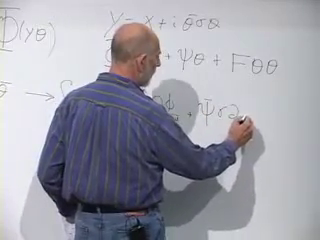
\includegraphics[width=0.76\textwidth]{lecture_09_figure_02.png}
\lectureframe{00:27:36.000}
\caption{手徵座標與分量展開；圖中標示了純量、費米子及輔助場項。}
\end{figure}

\section{\texorpdfstring{\(d^2\theta\)}{d2-theta}積分選出什麼}

相互作用與質量來自全純函數\(W(\Phi)\)，也就是超勢：
\begin{equation}
S_W
=
\int d^4x
\left[
\int d^2\theta\,W(\Phi)
+\mathrm{h.c.}
\right].
\label{eq:l9-superpotential-action}
\end{equation}
手徵表示式不獨立依賴\(\bar\theta\)，因此對全部四個反對易座標積分會得到零。\(d^2\theta\)積分則會選出其中的\(\theta^2\)分量。

先以一般函數之前的簡單例子說明組合方式，令\(W(\Phi)=\Phi^n\)。在
\begin{equation}
(\phi+\sqrt2\,\theta\psi+\theta^2F)^n,
\end{equation}
中，恰好得到兩個\(\theta\)的方式有兩種：可以選取一個\(F\theta^2\)，也可以選取兩個費米子因子。

\begin{classroomqa}
\audiencequestion{有多少項包含一個選定的\(F\theta^2\)，其餘因子則全是純量：是\(n-1\)個還是\(n\)個？\lecturetimestamp{00:31:33}}
\lecturerresponse{共有\(n\)項。\(n\)個因子中的任一個都可以提供\(F\theta^2\)，其餘\(n-1\)個因子則提供\(\phi\)。這些項的貢獻為\(nF\phi^{n-1}\)。}
\end{classroomqa}

\begin{classroomqa}
\audiencequestion{有多少種方式可由兩個因子提供兩個費米子？\lecturetimestamp{00:32:26}}
\lecturerresponse{共有\(\binom n2=n(n-1)/2\)種不計順序的選法。格拉斯曼縮併會決定相應的\(\psi\psi\)項。}
\end{classroomqa}

因此，按照講義中省略係數的記號，
\begin{equation}
\int d^2\theta\,\Phi^n+\mathrm{h.c.}
\;\leadsto\;
nF\phi^{n-1}
-\frac{n(n-1)}{2}\phi^{n-2}\psi\psi
+\mathrm{h.c.}
\label{eq:l9-power-extraction}
\end{equation}
此處的負號遵循標準的歸一化展開與格拉斯曼慣例；若採用不同慣例，表面上的符號可能有所不同。

\begin{classroomqa}
\audiencequestion{不含任何\(\theta\)的項\(\phi^n\)怎麼處理？\lecturetimestamp{00:33:10}}
\lecturerresponse{它確實出現在乘積中，但會被\(d^2\theta\)積分捨去。箭頭表示積分會選出\(\theta^2\)的係數；它不表示兩個完整表示式相等。}
\end{classroomqa}

\begin{figure}[H]
\centering
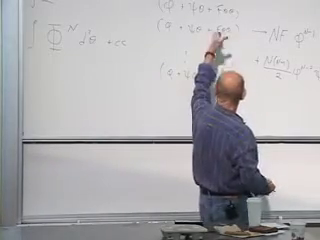
\includegraphics[width=0.82\textwidth]{lecture_09_figure_03.png}
\lectureframe{00:33:38.000}
\caption{重複的超場因子，以及表示取出它們的雙\(\theta\)分量、而非表示兩者相等的箭頭。}
\end{figure}

將帶有任意係數的各次冪加總後，組合因子便轉化為導數：
\begin{equation}
\int d^2\theta\,W(\Phi)+\mathrm{h.c.}
\;\leadsto\;
F W'(\phi)
-\frac12 W''(\phi)\psi\psi
+\mathrm{h.c.}
\label{eq:l9-W-components}
\end{equation}

\begin{classroomqa}
\audiencequestion{為什麼費米子項含有\(\phi^{n-2}\)，而不是\(\phi^{n-1}\)？\lecturetimestamp{00:36:32}}
\lecturerresponse{兩個因子已經提供費米子，剩下\(n-2\)個純量因子。因此係數是二階導數\(W''(\phi)\)的一半。}
\end{classroomqa}

費米子項相當重要：\(W''\)為常數時，它給出質量；\(W''\)依賴\(\phi\)時，它給出湯川相互作用。不過在分析真空時，輔助場項\(FW'\)提供了直接的資訊。

\section{消去輔助場}

整理出含有\(F\)的各項：
\begin{equation}
\mathcal L_F
=
F^\ast F
+F W'(\phi)
+F^\ast \overline{W'(\phi)}.
\label{eq:l9-LF}
\end{equation}
由於沒有\(\partial_\mu F\)項，完整的歐拉--拉格朗日方程
\begin{equation}
\partial_\mu
\frac{\partial\mathcal L}{\partial(\partial_\mu F)}
-
\frac{\partial\mathcal L}{\partial F}
=0
\end{equation}
會立即化為代數方程。將\(F\)與\(F^\ast\)視為獨立變數，可得
\begin{align}
\frac{\partial\mathcal L_F}{\partial F}
&=F^\ast+W'(\phi)=0,
&
\frac{\partial\mathcal L_F}{\partial F^\ast}
&=F+\overline{W'(\phi)}=0,
\label{eq:l9-F-eom}
\end{align}
因此
\begin{equation}
F^\ast=-W'(\phi),
\qquad
F=-\overline{W'(\phi)}.
\label{eq:l9-F-solution}
\end{equation}

\begin{figure}[H]
\centering
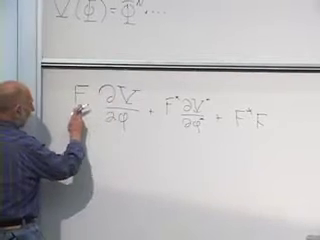
\includegraphics[width=0.82\textwidth]{lecture_09_figure_04.png}
\lectureframe{00:39:40.000}
\caption{板書遮擋移除後，完整的輔助場表示式及其代數運動方程一覽無遺。}
\end{figure}

\begin{classroomqa}
\audiencequestion{該導數應該對\(\phi\)取，而不是對黑板上寫的共軛場取嗎？\lecturetimestamp{00:41:21}}
\lecturerresponse{是的。修正後，式~\eqref{eq:l9-F-eom}中的共軛對便完整了：\(F^\ast=-W'(\phi)\)與\(F=-\overline{W'(\phi)}\)。}
\end{classroomqa}

代入式~\eqref{eq:l9-LF}可得
\begin{equation}
\mathcal L_F\big|_{\mathrm{on\ shell}}
=-|W'(\phi)|^2.
\end{equation}
由於純量拉格朗日量的形式是動能減去勢能，普通的純量勢為
\begin{equation}
\boxed{V(\phi,\phi^\ast)=|W'(\phi)|^2\ge0.}
\label{eq:l9-F-potential}
\end{equation}
這個\(V\)不是超勢。我們以\(W\)表示超空間中的全純函數，以\(V\)表示普通勢能。

\subsection{兩個直接例子}

採用標準的精確歸一化，
\begin{equation}
\begin{gathered}
W(\Phi)=\frac12m\Phi^2,\\
W'(\phi)=m\phi,
\qquad V=|m|^2|\phi|^2.
\end{gathered}
\label{eq:l9-quadratic-W}
\end{equation}
同一項也給出費米子質量
\(-\tfrac12m\psi\psi+\mathrm{h.c.}\)，因此超對稱破缺之前，純量與費米子的質量相同。

若取
\begin{equation}
W(\Phi)=\frac{g}{3}\Phi^3,
\end{equation}
則可得
\begin{equation}
\begin{gathered}
W'(\phi)=g\phi^2,
\qquad V=|g|^2|\phi|^4,\\
\mathcal L_{\mathrm{Yukawa}}
=-g\phi\psi\psi+\mathrm{h.c.}
\end{gathered}
\label{eq:l9-cubic-W}
\end{equation}
四純量頂點描述兩個純量的散射，而湯川項則是與之相應的超對稱項。

\section{兩種真空}

真空是\(V\)取極小值時的常數場構型；此時導數項為零。由於式~\eqref{eq:l9-F-potential}非負，可能的情況有兩種。

\subsection{零能量極小值}

若存在某個\(\phi_0\)滿足
\begin{equation}
W'(\phi_0)=0,
\end{equation}
則
\begin{equation}
V(\phi_0)=0,
\qquad
\langle F\rangle=0.
\label{eq:l9-unbroken-F}
\end{equation}
此真空具有超對稱性。這類似磁化強度為零的情況：沒有輔助場分量選定超空間方向。

\subsection{能量抬升的極小值}

若方程
\begin{equation}
W'(\phi)=0
\label{eq:l9-F-flatness}
\end{equation}
在極小值處沒有共同解，則
\begin{equation}
V_{\min}>0,
\qquad
\langle F\rangle\neq0,
\label{eq:l9-broken-F}
\end{equation}
超對稱便自發破缺。作用量仍具有超對稱性，但其最低能量態沒有。

\begin{figure}[H]
\centering
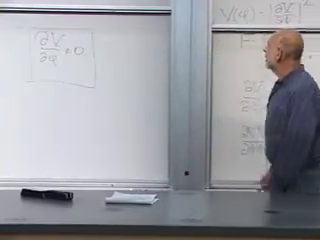
\includegraphics[width=0.88\textwidth]{lecture_09_figure_05.png}
\lectureframe{00:52:09.960}
\caption{板書同時列出正定的勢、\(F\)方程與真空條件，並呈現對稱的方程如何導出不具對稱性的解。}
\end{figure}

透過費米子變換，可以精確表述序參量的意義：
\begin{equation}
\delta\psi_\alpha
=
i\sqrt2
(\sigma^\mu\bar\epsilon)_\alpha\partial_\mu\phi
+\sqrt2\,\epsilon_\alpha F.
\label{eq:l9-fermion-transformation}
\end{equation}
對均勻真空而言，導數項為零。若\(\langle F\rangle\neq0\)，超對稱變換就會使費米子產生非零的常數位移，因此真空不可能保持不變。\editorialnote{方程~\eqref{eq:l9-fermion-transformation}是標準的分量形式，明確呈現講課中所說的超場分量會彼此變換。}

同樣的結論也可由超代數導出。在靜止系中，
\begin{equation}
\{Q_\alpha,Q_{\dot\alpha}^\dagger\}
=2\sigma^0_{\alpha\dot\alpha}H.
\end{equation}
取真空期望值後，真空能量可表示為超荷作用於真空所得各態的範數平方總和：
\begin{equation}
E_0\ge0,
\qquad
E_0=0
\ \Longleftrightarrow\
Q_\alpha|0\rangle
=Q_{\dot\alpha}^\dagger|0\rangle=0.
\label{eq:l9-algebra-vacuum-energy}
\end{equation}
因此，在剛性超對稱理論中，真空能為正與超對稱自發破缺是同一件事的兩面。

\begin{center}
\begin{tikzpicture}[x=1.2cm,y=1.0cm,>=Latex]
  \draw[->] (-3,0) -- (-0.2,0) node[right] {\(\phi\)};
  \draw[->] (-2.8,-0.15) -- (-2.8,2.1) node[above] {\(V\)};
  \draw[thick,teal!75!black,domain=-2.5:-0.5,samples=60]
    plot (\x,{0.65*(\x+1.5)^2});
  \fill (-1.5,0) circle (2pt);
  \node[below] at (-1.5,0) {\(F=0\)};
  \draw[->] (0.4,0) -- (3.2,0) node[right] {\(\phi\)};
  \draw[->] (0.6,-0.15) -- (0.6,2.1) node[above] {\(V\)};
  \draw[thick,orange!85!black,domain=0.9:2.9,samples=60]
    plot (\x,{0.55*(\x-1.9)^2+0.65});
  \fill (1.9,0.65) circle (2pt);
  \draw[dashed] (0.6,0.65) -- (1.9,0.65);
  \node[below] at (1.9,0.65) {\(F\neq0\)};
\end{tikzpicture}
\end{center}

\editorialnote{一個最簡單的例子是\(W=f\Phi\)；其中\(W'=f\)永不為零，而且\(V=|f|^2\)。這個單場例子具有平坦的純量方向；若要實現穩定的\(F\)項破缺，通常需要多個手徵場，例如 O'Raifeartaigh 型隱藏部門。}

\section{超對稱破缺會產生什麼}

\subsection{質量分裂}

鐵磁體的類比在此再次回到譜上。弱內部磁場會使原子能階分裂，卻不會改變原子的本質。同樣地，弱耦合傳遞的超對稱破缺序參量，會使原本同屬一個超多重態的玻色子與費米子質量分裂。

\begin{classroomqa}
\audiencequestion{超對稱會使哪些粒子彼此轉換，因此真空破缺超對稱時，這些粒子會失去質量簡併？\lecturetimestamp{00:51:40}}
\lecturerresponse{玻色子與費米子。當狀態不再遵循聯繫兩者的變換時，它們的質量便不必相等。}
\end{classroomqa}

單靠\(\langle F\rangle\)並不會造成質量分裂；還需要能將破缺效應傳遞至可見場的耦合。若這些耦合很弱，可見粒子仍能清楚辨認，質量分裂也遠小於大統一或普朗克尺度。若耦合很強，情況就像原子受到巨大磁場扭曲，變成細長而難以辨認的物體。

\subsection{戈德斯通費米子}

對於一般的破缺生成元，\(J|0\rangle\)會產生玻色型戈德斯通態。超荷是費米型的，會將玻色態轉變為費米態。由於真空被視為玻色態，破缺的超荷會產生一個費米型零能態：
\begin{equation}
Q_\alpha|0\rangle
\sim
|\widetilde G_\alpha,\mathbf k=0\rangle.
\label{eq:l9-goldstino}
\end{equation}
其傳播態是無質量外爾費米子，也就是戈德斯通費米子，或稱戈德斯通微子。

\begin{classroomqa}
\audiencequestion{若超對稱變換不使真空保持不變，會產生什麼新態？\lecturetimestamp{00:53:24}}
\lecturerresponse{無質量費米子。一般戈德斯通定理的模式依然成立，但費米型生成元會將玻色型真空轉變為戈德斯通費米子。}
\end{classroomqa}

因此，剛性超對稱自發破缺必然有兩種表徵：
\begin{equation}
\boxed{
V_{\min}>0
\qquad\text{and}\qquad
\text{a massless goldstino}.
}
\label{eq:l9-rigid-breaking-signatures}
\end{equation}

\section{隱藏部門}

將原子與鐵磁體視為兩個部門，是很有用的看法。鐵磁體形成序參量，原子感受到的則是從鐵磁體傳遞而來的場。耦合很弱時，操控原子幾乎不會激發磁振子，也很難直接探測磁性介質。因此鐵磁體是隱藏的，但可從微小的譜線分裂推知它的存在。

超對稱模型建構也採用相同的說法。隱藏部門中的額外場會形成非零的\(F\)項或\(D\)項期望值。稱為媒介機制的相互作用會將破缺效應傳至可見部門，並為超伴粒子產生軟質量。效應傳遞微弱，可以解釋為何可見理論在遠高於低能尺度的基本尺度上仍近似具有超對稱性，但低能下的玻色子--費米子質量並不完全簡併。

這種架構並非自動成立；它需要額外場、穩定的破缺真空，以及可受控的媒介機制。因此講課將現實中的超對稱破缺描述為複雜且多少有些牽強，而非最小模型必然導出的單一結果。

\section{引力會改變這兩種表徵}

\subsection{真空能成為引力源}

沒有引力時，將所有能量加上一個常數，不會改變非引力實驗的結果。有引力時，真空能量密度會以宇宙學常數的形式進入愛因斯坦方程。正的\(V_{\min}\)會驅動加速膨脹。若其尺度與超伴粒子質量所需的粒子物理尺度相當，所產生的曲率便會遠遠大於觀測值。

\begin{classroomqa}
\audiencequestion{納入引力後，正的非零真空能會對宇宙造成什麼影響？\lecturetimestamp{01:00:40}}
\lecturerresponse{它會像宇宙學常數一樣，驅動加速膨脹。若真空能處於一般粒子物理尺度，其效應就會大得令人無法接受。}
\end{classroomqa}

局域超對稱，也就是超引力，會改變正定平方和的公式。為便於掌握，標準的\(N=1\) \(F\)項勢能為
\begin{equation}
\begin{aligned}
V_F={}&e^{K/M_P^2}
\left(
K^{i\bar j}D_iW\,D_{\bar j}\overline W
-\frac{3|W|^2}{M_P^2}
\right),\\
D_iW={}&\partial_iW+\frac{\partial_iK}{M_P^2}W.
\end{aligned}
\label{eq:l9-sugra-potential}
\end{equation}
由於存在負項，原則上可以部分抵銷超對稱破缺所產生的正能量。剩餘部分可能形成很小的宇宙學常數。

\editorialnote{講課刻意只給出示意性的修正，並明確對普朗克質量的放置方式提出疑問。方程~\eqref{eq:l9-sugra-potential}列出具有 Kähler 勢\(K\)的手徵多重態所適用的標準公式；規範\(D\)項還會帶來額外的非負貢獻。這個公式並未解釋觀測到的極小值；這仍是宇宙學常數問題。}

\subsection{超希格斯機制}

第二個引力效應可從極化態的計數來理解。一個自旋為\(j\)的有質量粒子，在靜止系中有\(2j+1\)個自旋態。

\begin{classroomqa}
\audiencequestion{有質量且自旋為\(j\)的粒子有多少個自旋態？\lecturetimestamp{01:05:16}}
\lecturerresponse{\(2j+1\) 個。特別是，有質量的自旋 1 粒子有三個態；而無質量規範玻色子只有螺旋度 \(+1\) 和 \(-1\)。}
\end{classroomqa}

這是運動學上的差別。有質量粒子可以經由洛侖茲變換到達靜止系，再以不同方向運動，同時保持自旋取向，因此所有自旋投影都必須存在。無質量粒子無法被超越，也無法帶到靜止。因此它只能具有兩種極端螺旋度。

對電弱規範場而言，
\begin{equation}
\underbrace{(+1,-1)}_{\text{massless vector}}
+
\underbrace{(0)}_{\text{Goldstone}}
\longrightarrow
\underbrace{(+1,0,-1)}_{\text{massive vector}}.
\label{eq:l9-higgs-count}
\end{equation}

\begin{classroomqa}
\audiencequestion{有質量\(W\)或\(Z\)的縱向極化從何而來？\lecturetimestamp{01:08:50}}
\lecturerresponse{來自戈德斯通玻色子。它被規範場吸收，補足有質量自旋 1 表示所需的三個態。}
\end{classroomqa}

引力具有無質量自旋 2 的引力子。它的超對稱夥伴是無質量、自旋為\(\tfrac32\)的引力微子。

\begin{classroomqa}
\audiencequestion{引力子的自旋是多少？它的超對稱夥伴自旋又是多少？\lecturetimestamp{01:10:24}}
\lecturerresponse{引力子的自旋為\(2\)；費米子夥伴的自旋相差二分之一，為\(3/2\)。}
\end{classroomqa}

無質量引力微子的螺旋度為\(\pm\tfrac32\)；有質量引力微子還必須具有\(\pm\tfrac12\)。戈德斯通微子恰好提供這些缺少的態：
\begin{equation}
\begin{gathered}
\underbrace{\left(+\frac32,-\frac32\right)}_{\text{massless gravitino}}
\oplus
\underbrace{\left(+\frac12,-\frac12\right)}_{\text{goldstino}}\\
\Downarrow\\
\underbrace{\left(+\frac32,+\frac12,-\frac12,-\frac32\right)}_{\text{massive gravitino}}.
\end{gathered}
\label{eq:l9-super-higgs}
\end{equation}
這就是超希格斯機制。超對稱一旦成為局域對稱，戈德斯通微子便會被吸收，不再以獨立的無質量粒子出現。由此形成的引力微子透過引力作用，因此很難產生。

\section{轉換主題：為什麼選擇\texorpdfstring{\(SU(5)\)}{SU(5)}？}

接下來從超對稱形式體系轉向大統一。標準模型的規範群為
\begin{equation}
G_{\mathrm{SM}}
=SU(3)_c\times SU(2)_L\times U(1)_Y.
\label{eq:l9-sm-group}
\end{equation}
其三個因子分別描述色、弱同位旋與弱超荷。大統一要探討的是：這個乘積群是否是一個更大單群的剩餘子群，使表面上各自分離的粒子多重態與規範作用力都成為同一結構的一部分。此處要討論的最小候選群是\(SU(5)\)。

\subsection{群元素與生成元}

對於\(U\in SU(N)\)，
\begin{equation}
U^\dagger U=\mathbf1,
\qquad
\det U=1.
\label{eq:l9-SUN-def}
\end{equation}
第一個條件表示么正性；第二個條件則定義了「特殊」群。將無窮小群元素寫成
\begin{equation}
U=\mathbf1+i\epsilon G+\mathcal O(\epsilon^2).
\label{eq:l9-infinitesimal-U}
\end{equation}
么正性要求
\begin{equation}
G^\dagger=G,
\end{equation}
而
\begin{equation}
\det e^{i\epsilon G}
=e^{i\epsilon\operatorname{tr}G}=1
\end{equation}
則要求
\begin{equation}
\operatorname{tr}G=0.
\end{equation}
因此，生成元是無跡的厄米矩陣。

一個\(N\times N\)厄米矩陣含有\(N^2\)個實參數：\(N\)個實對角元，以及\(N(N-1)/2\)個複數非對角元。無跡條件會去掉一個參數。因此
\begin{equation}
\dim SU(N)=N^2-1,
\qquad
\dim SU(5)=24.
\label{eq:l9-SU5-dimension}
\end{equation}
作為比較，\(SU(2)\)有三個泡利生成元，\(SU(3)\)則有八個色生成元。

\section{\texorpdfstring{\(SU(5)\)}{SU(5)}中的標準模型基本組件}

將五維空間分成弱同位旋的二維區塊與色的三維區塊：
\begin{equation}
\mathbf5=\mathbf2\oplus\mathbf3.
\end{equation}
嵌入的生成元形式如下：
\begin{align}
T^a_L
&=
\begin{pmatrix}
\tfrac12\tau^a&0\\
0&0_{3\times3}
\end{pmatrix},
&& a=1,2,3,
\label{eq:l9-SU2-block}\\
T^A_c
&=
\begin{pmatrix}
0_{2\times2}&0\\
0&\tfrac12\lambda^A
\end{pmatrix},
&& A=1,\ldots,8.
\label{eq:l9-SU3-block}
\end{align}
泡利矩陣\(\tau^a\)生成弱\(SU(2)\)；蓋爾曼矩陣\(\lambda^A\)生成色\(SU(3)\)。由於兩個區塊互不重疊，這兩個子群彼此對易。

另一個對角生成元在每個區塊內都正比於單位矩陣，因此與兩者皆對易。在基本表示中，一種方便的雙倍超荷慣例為
\begin{equation}
T_Y^{(\mathbf5)}=
\operatorname{diag}
\left(
1,1,-\frac23,-\frac23,-\frac23
\right).
\label{eq:l9-hypercharge-generator}
\end{equation}
其跡為零：
\begin{equation}
1+1-3\left(\frac23\right)=0.
\end{equation}
共軛物質表示的本徵值符號相反：
\begin{equation}
Y_{\overline{\mathbf5}}
=
\operatorname{diag}
\left(
-1,-1,\frac23,\frac23,\frac23
\right),
\label{eq:l9-fivebar-hypercharge}
\end{equation}
這些數值就是講義中物質欄所列的值。整體符號與歸一化皆屬慣例；此處採用標準模型慣例
\begin{equation}
Q=T_3+\frac{Y}{2}.
\label{eq:l9-charge}
\end{equation}
方程~\eqref{eq:l9-SU2-block}--\eqref{eq:l9-hypercharge-generator}展示了
\begin{equation}
SU(3)_c\times SU(2)_L\times U(1)_Y
\subset SU(5).
\end{equation}

三個弱作用生成元、八個色生成元和一個超荷生成元，合計為\(12\)個，佔\(24\)個\(SU(5)\)生成元中的一半。\editorialnote{其餘十二個生成元位於非對角的\(2\times3\)區塊和\(3\times2\)區塊。它們所對應的規範玻色子會在夸克型分量與輕子型分量之間進行轉換；這正是後續將探討的重子數與輕子數改變相互作用的結構性起源。}

\begin{classroomqa}
\audiencequestion{哪些規範粒子對應於熟悉的子群生成元？\lecturetimestamp{01:31:05}}
\lecturerresponse{八個\(SU(3)\)生成元對應八個膠子。三個\(SU(2)\)生成元對應弱規範場；經過電弱混合後，這些場成為\(W^\pm\)，以及\(Z\)－光子系統中的一部分；\(U(1)\)場則提供另一個中性組合。}
\end{classroomqa}

\section{以左手場描述一代粒子}

聚焦於第一代；{\proseunicodefont μ}子／粲夸克／奇夸克代，以及{\proseunicodefont τ}子／頂夸克／底夸克代，也都遵循相同模式。最簡潔的計數方式，是將每個獨立的維爾場都視為左手場。右手粒子則以其左手電荷共軛場表示：
\begin{equation}
Q_L=(u_L,d_L),\quad
L_L=(\nu_{eL},e_L),\quad
u^c_L,\quad d^c_L,\quad e^c_L.
\end{equation}
它們的重數如下：
\begin{equation}
\underbrace{6}_{Q_L}
+
\underbrace{2}_{L_L}
+
\underbrace{3}_{u^c_L}
+
\underbrace{3}_{d^c_L}
+
\underbrace{1}_{e^c_L}
=15.
\label{eq:l9-fifteen-fields}
\end{equation}

\editorialnote{最小標準模型不包含獨立的右手中微子維爾場，因此場的數目為\(15\)。僅憑這項計數，不能據此斷言中微子是馬約拉納粒子。加入一個單態場\(\nu^c_L\)後，場的數目便成為\(16\)，並自然引向\(SO(10)\)，這已超出目前\(SU(5)\)構造的範圍。}

五維多重態必須將無色的弱二重態分量置於前兩個位置，並將有色的弱單態分量置於後三個位置。

\begin{classroomqa}
\audiencequestion{所提出的欄向量包含六個場，而不是五個嗎？\lecturetimestamp{01:36:14}}
\lecturerresponse{不是。第一輪寫下的上夸克已被刪去。這個欄向量包含中微子、電子，以及反下夸克的三種顏色態，總共五個分量。}
\end{classroomqa}

因此得到
\begin{equation}
\overline{\mathbf5}
=
\begin{pmatrix}
\nu_{eL}\\
e_L\\
d^c_{rL}\\
d^c_{gL}\\
d^c_{bL}
\end{pmatrix}.
\label{eq:l9-fivebar}
\end{equation}
\editorialnote{講義起初只稱它為五維多重態。依照標準的全左手\(SU(5)\)記號，其色與超荷指派顯示它屬於共軛表示\(\overline{\mathbf5}\)。}
前兩個分量在\(SU(2)_L\)變換下會改變，但不帶色荷。後三個分量在色變換下屬於反三重態，但都是弱單態。

\begin{classroomqa}
\audiencequestion{當所有場都寫成左手場時，哪些夸克帶有色荷，卻不帶弱\(SU(2)_L\)量子數？\lecturetimestamp{01:40:13}}
\lecturerresponse{右手夸克的電荷共軛場。對這個五分量多重態而言，依電荷判定，符合條件的是三個反下夸克場\(d^c_{r,g,b}\)。}
\end{classroomqa}

式~\eqref{eq:l9-fivebar}中的電荷總和為零：
\begin{equation}
0-1+\frac13+\frac13+\frac13=0.
\label{eq:l9-fivebar-charge-sum}
\end{equation}
這是必要的，因為電荷算符是\(SU(5)\)生成元的無跡組合。

\begin{classroomqa}
\audiencequestion{為什麼三個色分量是反下夸克，而不是反上夸克？\lecturetimestamp{01:43:38}}
\lecturerresponse{中微子和電子的總電荷為\(-1\)。三種顏色的反下夸克總電荷為\(+1\)，使總和為零。若換成三個反上夸克場，總電荷就會不對。}
\end{classroomqa}

剩下的十個左手場為
\begin{equation}
Q_L\;(6)
\oplus
u^c_L\;(3)
\oplus
e^c_L\;(1),
\end{equation}
它們恰好組成反對稱二階表示
\begin{equation}
\mathbf{10}\cong\wedge^2\mathbf5,
\qquad
\dim\wedge^2\mathbf5=\binom52=10.
\label{eq:l9-ten-preview}
\end{equation}
如何明確地將這些場配置於表示中，是下一講的任務。每一代標準模型粒子都符合這項數目上的吻合：
\begin{equation}
\overline{\mathbf5}\oplus\mathbf{10}
\end{equation}
這是\(SU(5)\)構想並非任意重新標記的第一個顯著證據。

\begin{classroomqa}
\audiencequestion{如果五重態和十重態是不同的表示，是否代表其中的粒子不能互相作用？\lecturetimestamp{01:46:14}}
\lecturerresponse{不會。群變換在各自的不可約表示內作用，因此不會直接將五重態中的成員變換成十重態中的成員。不過，這兩組場仍可透過發射與吸收共同的規範玻色子而互相作用，希格斯耦合也能連結它們。}
\end{classroomqa}

\section{回顧與展望}

本講追蹤了一個橫跨迥異尺度的相同模式。旋轉不變性使原子能階簡併；磁場背景則使能階分裂。鐵磁體會產生這樣的背景，同時使底層定律維持對稱；無能隙磁振子的存在，則顯示不對稱性出現在真空中。在手徵超對稱理論裡，輔助場的期望值扮演序參量的角色：
\begin{equation}
\begin{aligned}
\langle F\rangle=0
&\quad\Longleftrightarrow\quad
\text{unbroken supersymmetry},\\
\langle F\rangle\neq0
&\quad\Longrightarrow\quad
\text{spontaneous breaking}.
\end{aligned}
\end{equation}
在剛性超對稱下，對稱性破缺的真空具有正能量，會使超多重態分裂，並產生戈德斯通費米子。弱作用媒介機制促使人們引入隱藏部門；引力則使真空能成為宇宙學問題，並將戈德斯通費米子吸收進有質量的引力微子。

結尾的\(SU(5)\)構造開啟了一個新問題，並未將它解決。無跡厄米\(5\times5\)生成元包含標準模型的各個區塊，而前五個物質場恰好可嵌入為
\((\nu_e,e^-,d^c_r,d^c_g,d^c_b)\)。其餘十個場則位於反對稱表示中，尚待安排。這項尚未完成的嵌入，正是大統一理論真正開始之處。
